\section{Visión}
\begin{frame}\frametitle{Las imágenes como funciones}
Una imagen (en escala de grises) es una función $I(x,y)$ donde $x,y$ son variables discretas en coordenadas de imagen y la función $I$ es intensidad luminosa. Las imágenes también pueden considerarse como arreglos bidimensionales de números entre un mínimo y un máximo (usualmente 0-255).
\begin{figure}
  \centering
  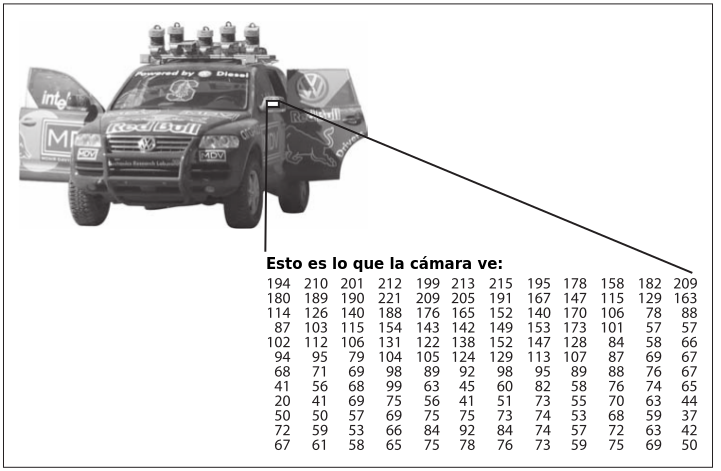
\includegraphics[width=0.45\textwidth]{Figures/representation_image.png}
\end{figure}
  Aunque formalmente una imagen es un mapeo $f:\mathbb{R}^2\rightarrow \mathbb{R}$, en la práctica, tanto $x,y$ como $I$ son varialbes discretas con valores entre un mínimo y un máximo.
\end{frame}

\begin{frame}\frametitle{Espacios de color}
  Las imágenes de color son funciones vectoriales $f:\mathbb{R}^2\rightarrow \mathbb{R}^3$ donde cada componente de la función se llama canal:
  \[I(x,y) = \left[\begin{tabular}{c}$r(x,y)$\\$g(x,y)$\\$b(x,y)$\end{tabular}\right]\]  
  Los espacios de color son diferentes formas de representar el color mediante la combinación de un conjunto de valores. 
  \begin{figure}
    \centering
    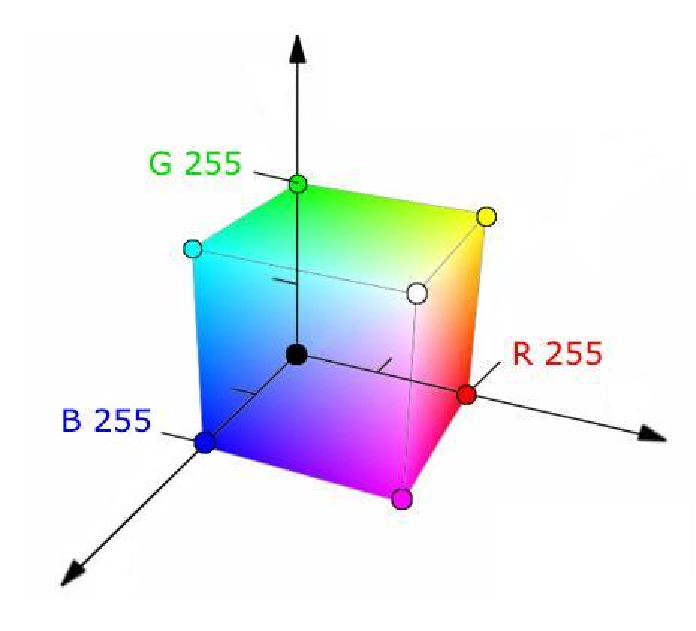
\includegraphics[width=0.33\textwidth]{Figures/RGB_model.pdf}
    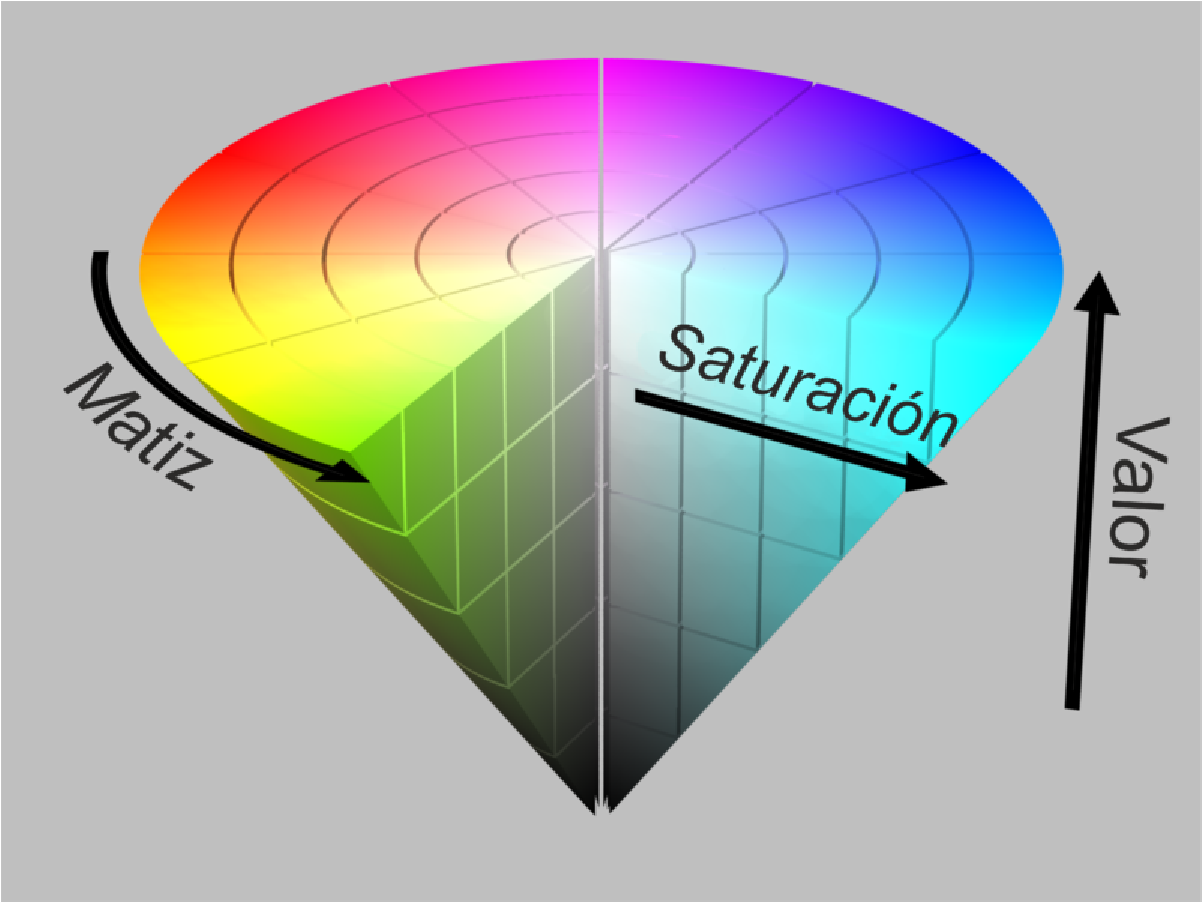
\includegraphics[width=0.33\textwidth]{Figures/hsv_space.pdf}
  \end{figure}
  En segmentación por color se recomienda más usar HSV, pues es más robusto ante cambios en la iluminación.
\end{frame}

\begin{frame}\frametitle{Nubes de puntos}
  Las nubes de puntos son conjuntos de vectores que representan puntos en el espacio. Estos vectores generalmente tienen información de posición $(x,y,z)$. También pueden contener información de color $(x,y,z,r,g,b)$.
  \begin{figure}
      \centering
      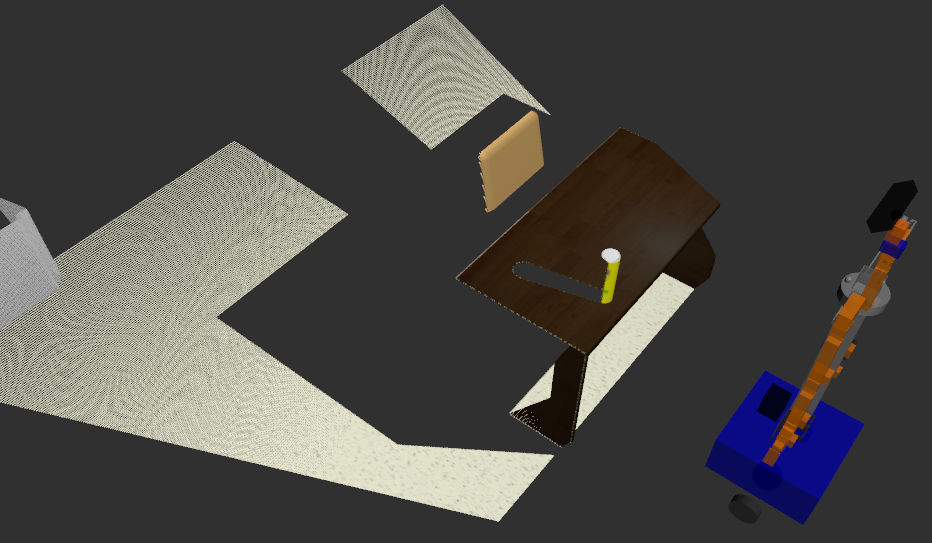
\includegraphics[width=0.5\textwidth]{Figures/CloudExample.png}
  \end{figure}
  Son útiles para determinar la posición en el espacio de los objetos reconocidos. 
\end{frame}

\begin{frame}\frametitle{OpenCV}
  \begin{itemize}
  \item OpenCV es un conjunto de bibliotecas que facilita la implementación de algoritmos de visión computacional.
  \item Se puede usar con diversos lenguajes: C++, Python, Java.
  \item En Python utiliza la biblioteca Numpy.
  \item Las imágenes se representan como matrices donde cada elemento puede ser un solo valor, o bien tres valores, dependiendo de si la imagen está en escala de grises o a color.
  \item La configuración más común es que cada pixel esté representado por tres bytes.
  \item Las nubes de puntos se representan también como matrices donde cada elemento es una terna de flotantes con la posición $(x,y,z)$.
  \end{itemize}
\end{frame}

\begin{frame}\frametitle{Segmentación por color}
  La segmentación de una imagen se refiere a obtener regiones significativas con ciertas características. En este caso, la característica es que estén en un cierto intervalo de color. Los pasos generales para esto son:
  \begin{enumerate}
  \item Transformación de la imagen del espacio BGR al HSV (función \texttt{cvtColor})
  \item Obtención de aquellos pixeles que están en un rango de color (función \texttt{inRange})
  \item Eliminación de \textit{outliers}, generalmente con operadores morfológicos (funciones \texttt{erode} y \texttt{dilate})
  \item Obtención del centroide de la región (funciones \texttt{findNonZero} y \texttt{mean})
  \item Si se dispone de una nube de puntos, se puede obtener la posición $(x,y,z)$ del centroide de la región segementada. 
  \end{enumerate}
\end{frame}

\begin{frame}[containsverbatim]\frametitle{Ejercicio 5}
  Modifique el archivo \texttt{catkin\_ws/src/exercises/scripts/color\_segmentation.py} para fijar los límites de color, superior e inferior, dependiendo del objeto que se desea segmentar. 
  \lstinputlisting[language=Python,firstnumber=17]{Codes/ColorSegmentation.py}
  Ejecute el comando:
  \begin{lstlisting}
    roslaunch bring_up path_planning.launch
  \end{lstlisting}
  Y en otra terminal ejecute el comando
  \begin{lstlisting}
    rosrun exercises color_segmentation.py
  \end{lstlisting}
\end{frame}

\begin{frame}\frametitle{Ejercicio 5}
  Utilizando la GUI, baje la cabeza del robot hasta que los objetos del escritorio estén en el campo visual:
  \begin{figure}
    \centering
    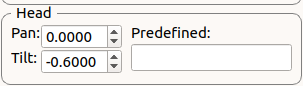
\includegraphics[width=0.35\textwidth]{Figures/Exercise5Gui1.png}
  \end{figure}
  Utilizando la GUI, ejecute la segmentación por color. Los objetos que se pueden segmentar son ``pringles'' o ``drink''.
  \begin{figure}
    \centering
    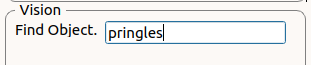
\includegraphics[width=0.35\textwidth]{Figures/Exercise5Gui2.png}
  \end{figure}
\end{frame}
